% Book pp. 151-158 (PDF pp. 152-159)
\section{Deriving the Equations of a Circle from Given Points}

\subsection{How to Find the Equation of the Circle Given the Endpoints of the Diameter}

\textit{Method 1:}

\textbf{Step 1:} Find the centre of the circle by finding the mid-point of the diameter.

\textbf{Step 2:} Calculate the length of the radius. This is half the diameter and is the
same as the distance between the centre and any of the endpoints of the diameter.

\textbf{Step 3:} Substitute the centre and the radius into the standard equation of the
circle.

\textbf{Step 4:} Simplify the resulting equation to achieve the desired result.

\textit{Method 2:}

An alternative method involves using the relationship between gradients of two
perpendicular lines.

Recall that if $m_1$ and $m_2$ are gradients of any two lines which intersect at right
angles, then $m_1 \times m_2 = -1$

Also, if one side of a triangle inscribed in a circle is a diameter, then the triangle
is right-angled. The angle opposite the diameter is the right angle. This property
of circles is illustrated in the diagram below.
\begin{center}
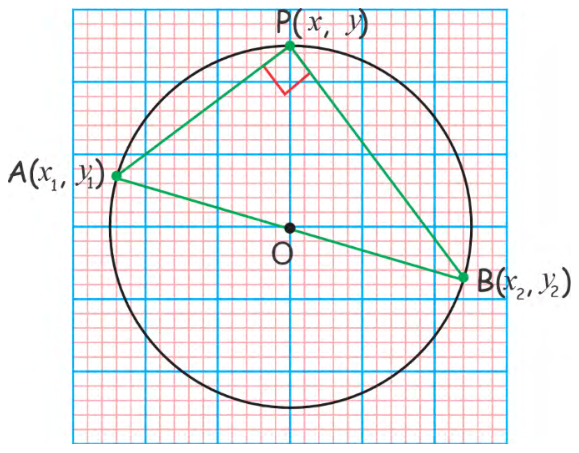
\includegraphics[width=0.42\linewidth]{figures/fig4-15.png}
\end{center}
\figcaption{4.15}{Graph of circle with centre O}

From the figure, $A(x_1, y_1)$ and $B(x_2, y_2)$ are the endpoints of the diameter and $P(x, y)$
is any point on the circumference of the circle. The angle opposite the diameter
is AOB$= 90^\circ$. This means that the product to the gradients of lines AP and BP is
equal to $-1$. Using this relation will generate the equation of the circle.
\booknote[S4-08]{the right angle is at P, so this should read APB $= 90^\circ$; O is
the centre.}
\begin{align*}
\text{Gradient } (m_1) \text{ of } |\text{AP}| &= \frac{y - y_1}{x - x_1} \\
\text{Gradient } (m_2) \text{ of } |\text{BP}| &= \frac{y - y_2}{x - x_2}
\end{align*}
Using $m_1 \times m_2 = -1$, we have
\[ \frac{y - y_1}{x - x_1} \times \frac{y - y_2}{x - x_2} = -1 \]

\begin{example}{Example 4.7}
The endpoints of the diameter of a circle are (-2, 2) and (4, -6).

Find the;
\begin{enumerate}
  \item[a.] radius and centre of the circle
  \item[b.] general equation of the circle.
\end{enumerate}

\solution
The graph below shows a sketch of the circle.
\begin{center}
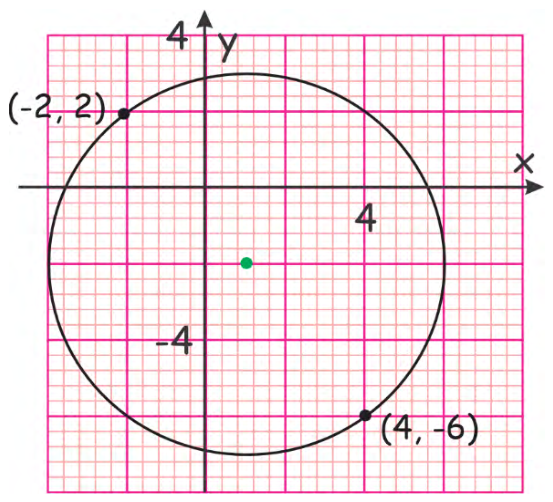
\includegraphics[width=0.42\linewidth]{figures/fig4-16.png}
\end{center}
\figcaption{4.16}{Graph of circle with diameter (-2, 2) and (4, -6)}

\textit{Method 1:}
\begin{enumerate}
  \item The centre is equal to the mid-point of the endpoints of the diameter
  \item Midpoint $= \frac{1}{2}(-2 + 4, 2 + (-6))$
  \item $= \frac{1}{2}(2, -4)$
  \item $= \left(\frac{2}{2}, -\frac{4}{2}\right) = \left(1, -2\right)$
\end{enumerate}
\booknote[S4-07]{the four lines of this working are numbered 1.\ to 4.\ in the
book, as if they were separate parts.}

Radius is the distance between the centre and any of the endpoint/point on the
circumference.
\begin{align*}
r &= \sqrt{(-6 - (-2))^2 + (4 - 1)^2} \\
r &= \sqrt{(-4)^2 + 3^2} \\
r &= \sqrt{16 + 9} \\
&= \sqrt{25} = 5
\end{align*}
Using $(x - h)^2 + (y - k)^2 = r^2$, we have:
\begin{align*}
(x - 1)^2 + (y - (-2))^2 &= 5^2 \\
(x - 1)^2 + (y + 2)^2 &= 25 \\
x^2 - 2x + 1 + y^2 + 4y + 4 &= 25 \\
x^2 + y^2 - 2x + 4y + 5 &= 25 \\
x^2 + y^2 - 2x + 4y + 5 - 25 &= 0 \\
\boldsymbol{x^2 + y^2 - 2x + 4y - 20} &= \boldsymbol{0}
\end{align*}

\textit{Method 2:}

Alternatively, let any point on the circumference of the circle be P(x, y) as shown
in the figure below.
\begin{center}
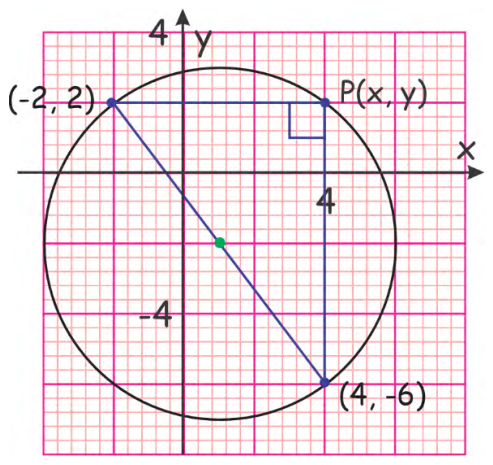
\includegraphics[width=0.4\linewidth]{figures/fig4-17.png}
\end{center}
\figcaption{4.17}{Graph of circle with diameter (-2, 2) and (4, -6)}

The gradient of the line connecting (-2, 2) and $(x, y) = \dfrac{-2}{x - (-2)} = \dfrac{y - 2}{x + 2}$
\booknote[S4-09]{the first numerator is printed as $-2$; it should be $y - 2$, as
the second fraction shows.}

The gradient of the line connecting (4, -6) and $(x, y) = \dfrac{y - (-6)}{x - 4} = \dfrac{y + 6}{x - 4}$

Since the two lines intersect at $90^\circ$,
\begin{align*}
\left(\frac{y - 2}{x + 2}\right) \times \left(\frac{y + 6}{x - 4}\right) &= -1 \\
\frac{(y - 2)(y + 6)}{(x + 2)(x - 4)} &= -1 \\
\frac{y^2 + 6y - 2y - 12}{x^2 - 4x + 2x - 8} &= -1 \\
\frac{y^2 + 4y - 12}{x^2 - 2x - 8} &= -\frac{1}{1}
\end{align*}
Cross multiply:
\begin{align*}
y^2 + 4y - 12 &= -1(x^2 - 2x - 8) \\
y^2 + 4y - 12 &= -x^2 + 2x + 8
\end{align*}
Regroup the terms:
\begin{align*}
y^2 + x^2 - 2x + 4y - 12 - 8 &= 0 \\
\boldsymbol{y^2 + x^2 - 2x + 4y - 20} &= \boldsymbol{0}
\end{align*}
\end{example}

\subsection{Equation of a Circle Given Three Points on the Circumference of the Circle}

\textit{Method 1:}

Substitute each of the points into the general equation of the circle
$(x^2 + y^2 + 2gx + 2fy + c = 0)$.

This results in 3 simultaneous equations with 3 unknowns to be solved for $g$, $f$
and $c$.

\textit{Method 2}:

Alternatively, follow the following steps.

\textbf{Step 1:} Find the equation of the perpendicular bisectors of any two of the chords.

In the Figure 4.18 A, B and C are points on the circumference of the circle.
\begin{center}
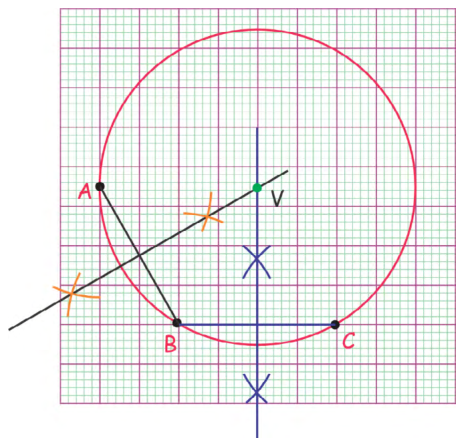
\includegraphics[width=0.38\linewidth]{figures/fig4-18.png}
\end{center}
\figcaption{4.18}{Graph of circle with equation $(x^2 + y^2 + 2gx + 2fy + c = 0)$}

\textbf{Step 2:} Solve the equations obtained in step 1 simultaneously. This will give the
coordinates of the centre of the circle.

\textbf{Step 3:} Using the centre and any point on the circumference, calculate the radius.

\textbf{Step 4:} Use the radius and the centre to calculate the equation of the circle.

\begin{example}{Example 4.8}
Find the equation of the circle which satisfies the points (2, -4), (-6, 4) and (2, 12).

\solution
\textit{Method 1}:

In the diagram below, A, B and C are points on the circumference of the circle.
The perpendicular bisectors of chords AB and BC intersect at point V. Point V is
the centre of the circle.
\begin{center}
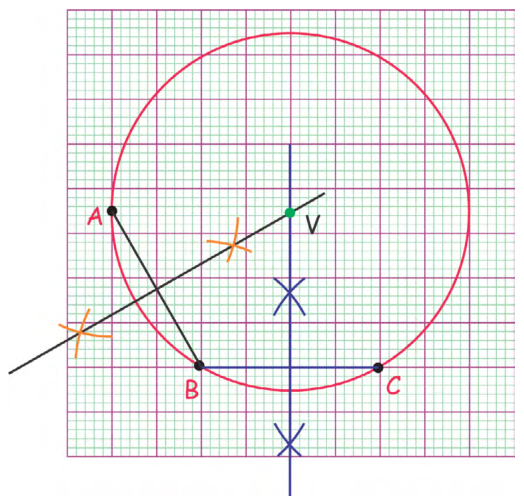
\includegraphics[width=0.42\linewidth]{figures/fig4-19.png}
\end{center}
\figcaption{4.19}{Graph of circle with points (2, -4), (-6, 4) and (2, 12)}

Substitute the points into the general equation of the circle.

Substituting (-6, 4) into $x^2 + y^2 + 2gx + 2fy + c = 0$ gives:
\begin{align*}
(-6)^2 + 4^2 + 2g(-6) + 2f(4) + c &= 0 \\
36 + 16 - 12g + 8f + c &= 0 \\
-12g + 8f + c &= -52 \ldots\ldots\ldots\ldots\ldots\ldots\ldots\ldots..(1)
\end{align*}
Substituting (2, 12) into the same equation:
\begin{align*}
(2)^2 + (12)^2 + 2g(2) + 2f(12) + c &= 0 \\
4 + 144 + 4g + 24f + c &= 0 \\
4g + 24f + c &= -148 \ldots\ldots\ldots\ldots\ldots\ldots\ldots\ldots\ldots...(2)
\end{align*}
Substituting (2, -4) into the same equation:
\begin{align*}
(2)^2 + (-4)^2 + 2g(2) + 2f(-4) + c &= 0 \\
4 + 16 + 4g - 8f + c &= 0 \\
4g - 8f + c &= -20 \ldots\ldots\ldots\ldots\ldots\ldots\ldots\ldots\ldots\ldots\ldots. (3)
\end{align*}
Subtract (2) from (3). That is (3) -- (2)
\begin{align*}
(4g - 8f + c) - (4g + 24f + c) &= -20 - (-148) \\
4g - 8f + c - 4g - 24f - c &= -20 + 148 \\
-32f &= 128 \\
f &= -\frac{128}{32} = -4
\end{align*}
Subtract (1) from (2):
\begin{align*}
(4g + 24f + c) - (-12g + 8f + c) &= -148 - (-52) \\
4g + 24f + c + 12g - 8f - c &= -148 + 52 \\
16g + 16f &= -96 \\
16g + 16(-4) &= -96 \\
16g - 64 &= -96 \\
16g &= -96 + 64 \\
\frac{16g}{16} &= -\frac{32}{16} \\
g &= -2
\end{align*}
Substitute $g = -2$ and $f = -4$ into (3):
\begin{align*}
4(-2) - 8(-4) + c &= -20 \\
-8 + 32 + c &= -20 \\
c &= -20 + 8 - 32 \\
c &= -44
\end{align*}
Finally, substitute $g$, f and c into the general equation.

$x^2 + y^2 + 2(-2)x + 2(-4)y - 44 = 0$

$\boldsymbol{x^2 + y^2 - 4x - 8y - 44 = 0}$ gives the equation of the circle which satisfies
$(2, -4)$, $(-6, 4)$ and $(2, 12)$.

\textit{Method 2}:

First plot the points on the x-y plane and connect the points with chords.
\begin{center}
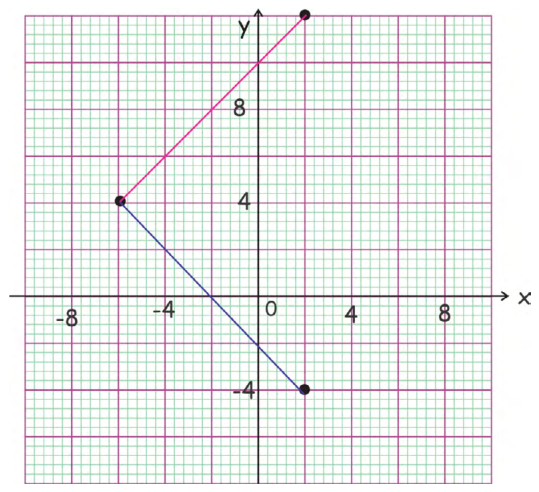
\includegraphics[width=0.42\linewidth]{figures/fig4-20.png}
\end{center}
\figcaption{4.20}{Graph of the $x$-$y$ plane}

Mid-point of $(-6, 4)$ and $(2, 12)$ is $\left(\dfrac{-6 + 2}{2}, \dfrac{4 + 12}{2}\right) = \left(-2, 8\right)$

The gradient of the line connecting the points $(-6, 4)$ and $(2, 12)$ is
\[ \frac{12 - 4}{2 - (-6)} = \frac{8}{8} = 1 \]
The gradient of the perpendicular bisector is $-1$

The equation of the perpendicular bisector is $y - 8 = -1(x - (-2))$
\begin{align*}
y &= -1(x + 2) + 8 \\
y &= -x - 2 + 8 \\
y &= -x + 6 \ldots\ldots\ldots\ldots\ldots\ldots\ldots\ldots.(1)
\end{align*}
Mid-point of $(-6, 4)$ and $(2, -4)$ is $\left(\dfrac{-6 + 2}{2}, \dfrac{4 - 4}{2}\right) = \left(-2, 0\right)$

The gradient of the line connecting the points $(-6, 4)$ and $(2, -4)$ is
\[ \frac{-4 - 4}{2 - (-6)} = \frac{-8}{8} = -1 \]
The gradient of the perpendicular bisector is 1

The equation of the perpendicular bisector is $y - 0 = 1(x - (-2))$
\begin{align*}
y &= (x + 2) \\
y &= x + 2 \\
y &= x + 2 \ldots\ldots\ldots\ldots\ldots\ldots\ldots\ldots.(2)
\end{align*}
Add equation 1 to equation 2:
\begin{align*}
y + y &= -x + x + 6 + 2 \\
2y &= 8 \\
y &= 4
\end{align*}
Substitute $y = 4$ into equation 2 and solve for $x$:
\begin{align*}
4 &= x + 2 \\
x &= 4 - 2 \\
x &= 2
\end{align*}
This means the coordinates of the centre of the circle is (2, 4).

The distance between the centre and any point on the circle's circumference gives
the radius.
\begin{align*}
\text{Distance between (2, 4) and (2, 12)} = r &= \sqrt{(2 - 2)^2 + (12 - 4)^2} \\
&= \sqrt{0^2 + 8^2} \\
&= \sqrt{64} \\
&= 8
\end{align*}
Finally, substitute the centre, (2, 4), and the radius, 8, into the standard equation
of the circle.
\begin{align*}
(x - 2)^2 + (y - 4)^2 &= 8^2 \\
x^2 - 4x + 4 + y^2 - 8y + 16 &= 64 \\
x^2 + y^2 - 4x - 8y + 20 - 64 &= 0 \\
\boldsymbol{x^2 + y^2 - 4x - 8y - 44} &= \boldsymbol{0}
\end{align*}
A construction of the circle is shown below
\begin{center}
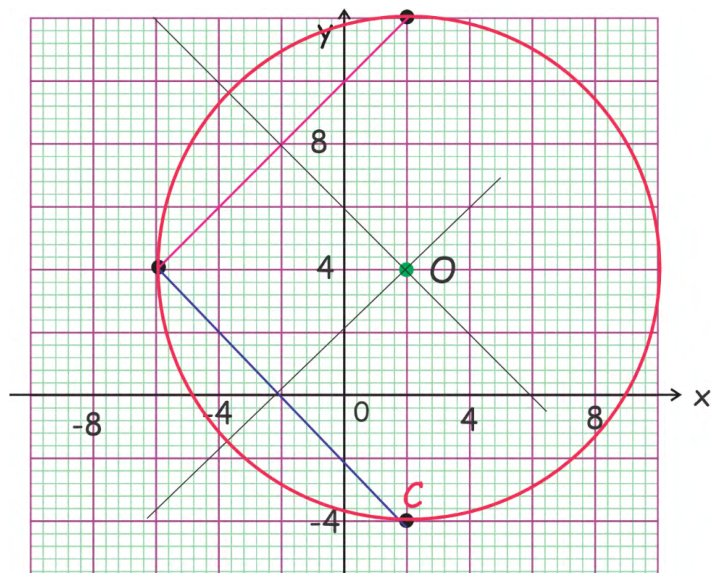
\includegraphics[width=0.55\linewidth]{figures/fig4-21.jpg}
\end{center}
\figcaption{4.21}{Graph of circle $x^2 + y^2 - 4x - 8y - 44 = 0$}
\end{example}
